\documentclass[a4paper,11pt]{article}


\usepackage{amsmath,amsfonts,amsthm,a4wide}
\usepackage{graphicx}
\usepackage[super]{nth}



\begin{document}
\begin{center}
University of Toronto at Scarborough\\[0.1in]
{\bf CSCC73H3 Algorithm Design and Analysis, FALL 2018} \\[0.1in]
{\large{\bf Assignment No.1: Greedy Scheduling}}\\[0.1in]
{\bf DUE:} September 22, 2018, at 11:59 pm
\end{center}


\vspace{0.1in}
\noindent
{\bf Student ID:} 1005642654 \\[0.15in]
{\bf Student Name:} KyooSik Lee
\vspace{0.3in}

\vspace{0.3in}
\begin{enumerate}

\item {\bf Description}

My greedy algorithm is to schedule longest second job first. 

{\bf Complexity}

The complexity of my algorithm is $O(n\log{}n)$ because it uses merge sort on second jobs.

{\bf Correctness}

Changing one of the optimal schedules to my greedy schedule by swapping jobs without enlarging total time ensures that my greedy schedule is optimal.

First, let's consider an optimal solution $O$, which is scheduled from $j_1$ to $j_n$. Then we have a job $j_k$ such that $j_k$'s finish time is identical to total finish time. (Figure 1)


\begin{figure}[hbt]
	\centering
	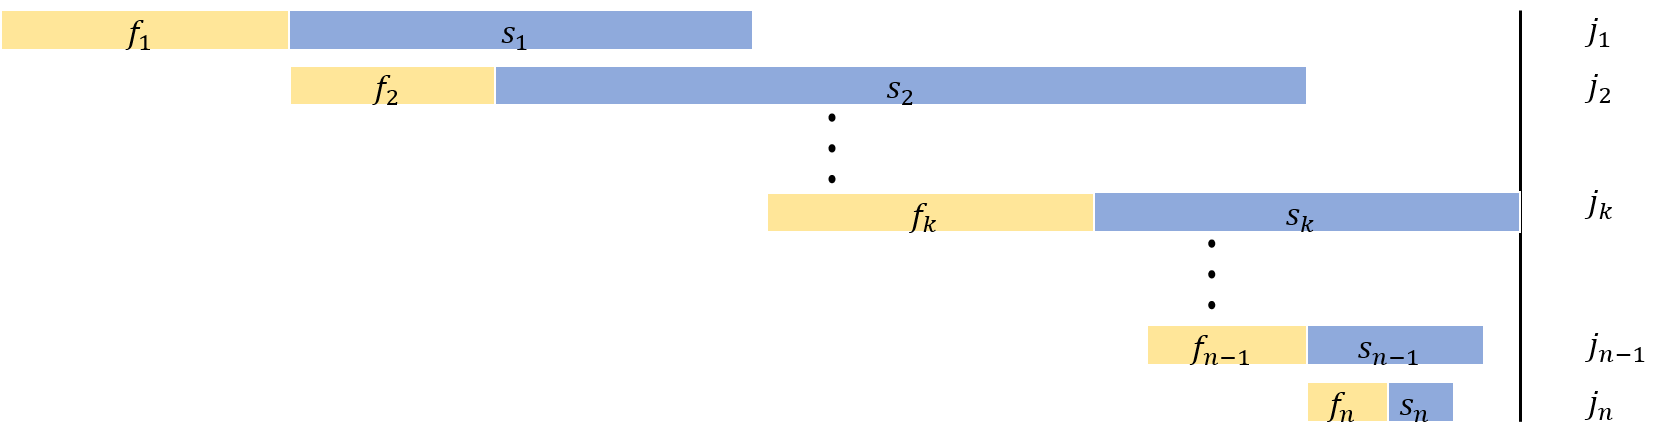
\includegraphics[scale=0.45]{figure1.png}
	\caption{Optimal Schedule $O$}
\end{figure}

Then $s_i(i\in \{1, 2\dots,k-1\})$ is bigger or equal to $s_k$. If not, swap $j_i$ with $j_k$, and it will decrease the total time, which contradicts that $O$ is an optimal schedule.

In the same sense, $s_i(i\in \{k+1,k+2\dots,n\}$) is strictly smaller than $s_k$. If not, it contradicts to the fact that $j_k$ is the one whose finish time is identical to total finish time.

Then we divide the jobs into two set $S_1=\{{j_1, j_2, ..., j_{k-1}}\}$ and $S_2=\{{j_{k+1}, j_{k+2}, ... j_n}$\}.

Now we do what we did on set ${\{j_1,j_2,...,j_n\}}$ to $S_1$ and $S_2$. 
The only difference is that now we can actually swap two jobs to reduce the total time of both sets. 
Note that reducing time of $S_1$ and $S_2$ does not affect to total finish time.
Doing this procedure recurrently on resulted two subsets of each procedure will sort $O$ by it's second job time.
Then the changed $O$ is identical to my greedy solution, making my greedy algorithm correct.



\pagebreak

\item 

{\bf Description}

My greedy algorithm is to schedule the earliest finish time first on different time bases.

This description will use a 24-hour system. 

First, sort the job by it's finish time. (Figure 2)

\begin{figure}[hbt]
	\centering
	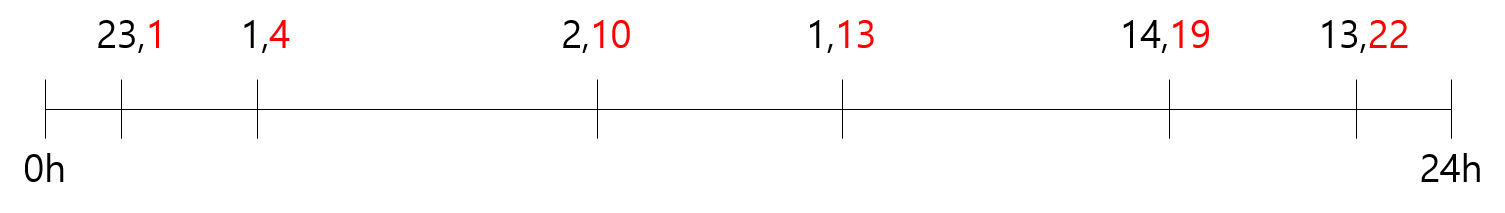
\includegraphics[scale=0.4]{figure2.png}
	\caption{Sorted Job List}
\end{figure}
Then make a circular singly linked list in growing finish time.(Figure 3)

\begin{figure}[hbt]
	\centering
	
\includegraphics[scale=0.4]{figure3.png}
	\caption{Circular Singly Linked List}
\end{figure}

Begin with the head node. Start a procedure by accepting the first node. 
Then iterate $n+1$ times. 
While iterating, accept the nodes that do not conflict with most previously accepted node.
After ${n+1}^{\text{th}}$ iteration, the iterator will sit on the next node of the node we started(of course, do not accept last two nodes).
Store the accepted node list in memory and start over the procedure from the current node with new list for accepted nodes. 
After total $n$ procedures, the iterator will sit on the head node we started.
After the procedures, find the list(s) that has maximum number of intervals.
That list(s) is my greedy solution.

{\bf Complexity}

Sorting the job list by it's finish time will take $O(n\log{}n)$ using merge sort.

Making the circular singly linked list will take $O(n)$ time.

Iterating the linked list will take $O(n^2)$ time, because there are $n^2+n$ iterations.

Finding the list that has maximum number of intervals will take $O(n)$ time.

In total the complexity of my Algorithm is O$(n^2)$.

{\bf Correctness}

Let's say we have an optimal solution $O$.
Pick any interval of $O$, label it $i_1$ and label each interval of $O$ in timing order($i_2, i_3, ..., i_n$).
From my algorithm's storage, find a list that starts with $i_1$(the storage has every list that starts with any interval).
Then compare the list with $O$. (Figure 4)

\begin{figure}[hbt]
	\centering
	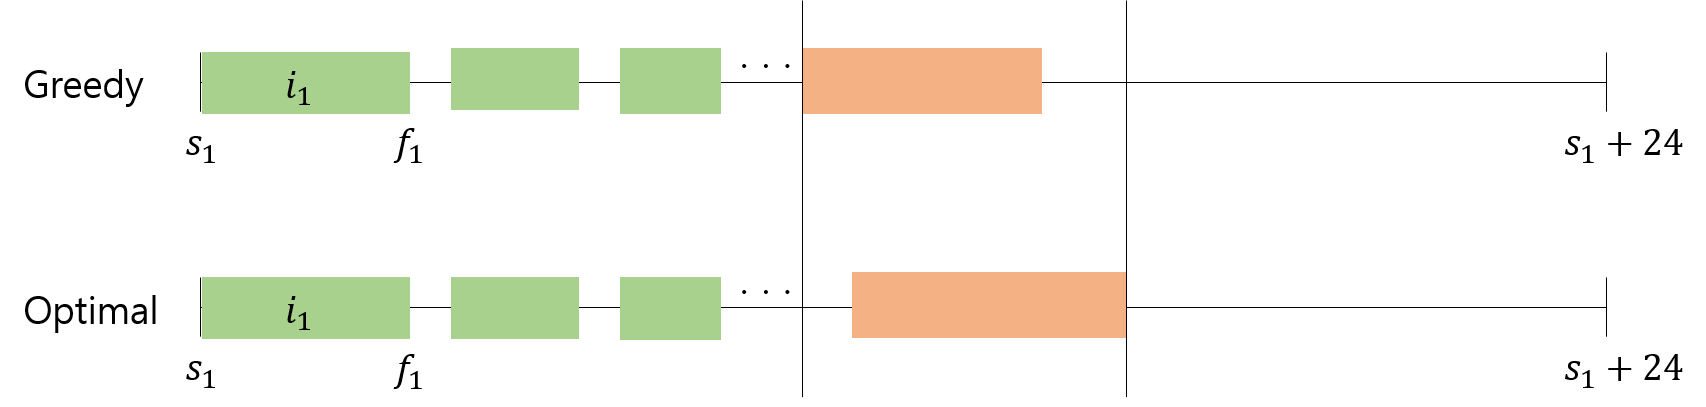
\includegraphics[scale=0.4]{figure4.png}
	\caption{Greedy Algorithm \& Optimal Algorithm}
\end{figure}
It is evident that the intervals that overlap with $i_1$ are neither in optimal nor greedy solution.
If we rule out the intervals that overlap with $i_1$, this problem is identical to the problem that was covered in class.

By the algorithm that was covered in class, we know that $G$ has same number of intervals as $O$ which makes $G$ an optimal solution.

Therefore my greedy algorithm is correct.
\end{enumerate}



\end{document}
